\documentclass[twoside]{book}

% Packages required by doxygen
\usepackage{fixltx2e}
\usepackage{calc}
\usepackage{doxygen}
\usepackage[export]{adjustbox} % also loads graphicx
\usepackage{graphicx}
\usepackage[utf8]{inputenc}
\usepackage{makeidx}
\usepackage{multicol}
\usepackage{multirow}
\PassOptionsToPackage{warn}{textcomp}
\usepackage{textcomp}
\usepackage[nointegrals]{wasysym}
\usepackage[table]{xcolor}

% Font selection
\usepackage[T1]{fontenc}
\usepackage[scaled=.90]{helvet}
\usepackage{courier}
\usepackage{amssymb}
\usepackage{sectsty}
\renewcommand{\familydefault}{\sfdefault}
\allsectionsfont{%
  \fontseries{bc}\selectfont%
  \color{darkgray}%
}
\renewcommand{\DoxyLabelFont}{%
  \fontseries{bc}\selectfont%
  \color{darkgray}%
}
\newcommand{\+}{\discretionary{\mbox{\scriptsize$\hookleftarrow$}}{}{}}

% Page & text layout
\usepackage{geometry}
\geometry{%
  a4paper,%
  top=2.5cm,%
  bottom=2.5cm,%
  left=2.5cm,%
  right=2.5cm%
}
\tolerance=750
\hfuzz=15pt
\hbadness=750
\setlength{\emergencystretch}{15pt}
\setlength{\parindent}{0cm}
\setlength{\parskip}{3ex plus 2ex minus 2ex}
\makeatletter
\renewcommand{\paragraph}{%
  \@startsection{paragraph}{4}{0ex}{-1.0ex}{1.0ex}{%
    \normalfont\normalsize\bfseries\SS@parafont%
  }%
}
\renewcommand{\subparagraph}{%
  \@startsection{subparagraph}{5}{0ex}{-1.0ex}{1.0ex}{%
    \normalfont\normalsize\bfseries\SS@subparafont%
  }%
}
\makeatother

% Headers & footers
\usepackage{fancyhdr}
\pagestyle{fancyplain}
\fancyhead[LE]{\fancyplain{}{\bfseries\thepage}}
\fancyhead[CE]{\fancyplain{}{}}
\fancyhead[RE]{\fancyplain{}{\bfseries\leftmark}}
\fancyhead[LO]{\fancyplain{}{\bfseries\rightmark}}
\fancyhead[CO]{\fancyplain{}{}}
\fancyhead[RO]{\fancyplain{}{\bfseries\thepage}}
\fancyfoot[LE]{\fancyplain{}{}}
\fancyfoot[CE]{\fancyplain{}{}}
\fancyfoot[RE]{\fancyplain{}{\bfseries\scriptsize Generated by Doxygen }}
\fancyfoot[LO]{\fancyplain{}{\bfseries\scriptsize Generated by Doxygen }}
\fancyfoot[CO]{\fancyplain{}{}}
\fancyfoot[RO]{\fancyplain{}{}}
\renewcommand{\footrulewidth}{0.4pt}
\renewcommand{\chaptermark}[1]{%
  \markboth{#1}{}%
}
\renewcommand{\sectionmark}[1]{%
  \markright{\thesection\ #1}%
}

% Indices & bibliography
\usepackage{natbib}
\usepackage[titles]{tocloft}
\setcounter{tocdepth}{3}
\setcounter{secnumdepth}{5}
\makeindex

% Hyperlinks (required, but should be loaded last)
\usepackage{ifpdf}
\ifpdf
  \usepackage[pdftex,pagebackref=true]{hyperref}
\else
  \usepackage[ps2pdf,pagebackref=true]{hyperref}
\fi
\hypersetup{%
  colorlinks=true,%
  linkcolor=blue,%
  citecolor=blue,%
  unicode%
}

% Custom commands
\newcommand{\clearemptydoublepage}{%
  \newpage{\pagestyle{empty}\cleardoublepage}%
}

\usepackage{caption}
\captionsetup{labelsep=space,justification=centering,font={bf},singlelinecheck=off,skip=4pt,position=top}

%===== C O N T E N T S =====

\begin{document}

% Titlepage & ToC
\hypersetup{pageanchor=false,
             bookmarksnumbered=true,
             pdfencoding=unicode
            }
\pagenumbering{alph}
\begin{titlepage}
\vspace*{7cm}
\begin{center}%
{\Large CS F214 Assignment Part 1 \\[1ex]\large v1.\+0 }\\
\vspace*{1cm}
{\large Generated by Doxygen 1.8.14}\\
\end{center}
\end{titlepage}
\clearemptydoublepage
\pagenumbering{roman}
\tableofcontents
\clearemptydoublepage
\pagenumbering{arabic}
\hypersetup{pageanchor=true}

%--- Begin generated contents ---
\chapter{CS F214 Assignment Part 1}
\label{index}\hypertarget{index}{}\hypertarget{index_Authors}{}\section{Authors}\label{index_Authors}

\begin{DoxyEnumerate}
\item Kunal Verma (2017\+A7\+P\+S0120H)
\item Sandesh Thakar (2017\+A7\+P\+S0181H)
\item Kushagra Srivastava (2017\+A7\+P\+S0146H)
\end{DoxyEnumerate}\hypertarget{index_Task}{}\section{Task}\label{index_Task}
Making a propositional logic proof checker, implementing the functionalties of\+:
\begin{DoxyEnumerate}
\item Premise
\item A\+ND Introduction ($^\wedge$i)
\item A\+ND Elimination (1 and 2) ($^\wedge$e)
\item OR Introduction (1 and 2) (Vi)
\item Implication Elimination ($>$e)
\end{DoxyEnumerate}\hypertarget{index_Assumptions}{}\section{Assumptions}\label{index_Assumptions}

\begin{DoxyEnumerate}
\item The expression should be perfectly paranthesized ~\newline
 Example 1\+: (a$^\wedge$b) is perfectly paranthesized while a$^\wedge$b is not ~\newline
 Example 2\+: (($\sim$p)$^\wedge$q) is perfectly paranthesized while ($\sim$p$^\wedge$q) is not
\item There should be no spaces within any line of proof
\end{DoxyEnumerate}\hypertarget{index_Sample}{}\section{Sample}\label{index_Sample}
Input ~\newline
 2 ~\newline
 a/P ~\newline
 (a\+Vb)/\+Vi1/1 ~\newline
 Output ~\newline
 Valid \mbox{\hyperlink{class_proof}{Proof}} 
\chapter{Class Index}
\section{Class List}
Here are the classes, structs, unions and interfaces with brief descriptions\+:\begin{DoxyCompactList}
\item\contentsline{section}{\mbox{\hyperlink{class_and_elimination}{And\+Elimination}} }{\pageref{class_and_elimination}}{}
\item\contentsline{section}{\mbox{\hyperlink{class_and_introduction}{And\+Introduction}} }{\pageref{class_and_introduction}}{}
\item\contentsline{section}{\mbox{\hyperlink{class_implies_elimination}{Implies\+Elimination}} }{\pageref{class_implies_elimination}}{}
\item\contentsline{section}{\mbox{\hyperlink{class_or_introduction}{Or\+Introduction}} }{\pageref{class_or_introduction}}{}
\item\contentsline{section}{\mbox{\hyperlink{class_proof}{Proof}} }{\pageref{class_proof}}{}
\end{DoxyCompactList}

\chapter{File Index}
\section{File List}
Here is a list of all files with brief descriptions\+:\begin{DoxyCompactList}
\item\contentsline{section}{C\+:/\+Users/\+Kunal/\+Desktop/\+Part2u/\+Part2/\mbox{\hyperlink{andelimination_8h}{andelimination.\+h}} }{\pageref{andelimination_8h}}{}
\item\contentsline{section}{C\+:/\+Users/\+Kunal/\+Desktop/\+Part2u/\+Part2/\mbox{\hyperlink{andintroduction_8h}{andintroduction.\+h}} }{\pageref{andintroduction_8h}}{}
\item\contentsline{section}{C\+:/\+Users/\+Kunal/\+Desktop/\+Part2u/\+Part2/\mbox{\hyperlink{implieselimination_8h}{implieselimination.\+h}} }{\pageref{implieselimination_8h}}{}
\item\contentsline{section}{C\+:/\+Users/\+Kunal/\+Desktop/\+Part2u/\+Part2/\mbox{\hyperlink{main_8cpp}{main.\+cpp}} }{\pageref{main_8cpp}}{}
\item\contentsline{section}{C\+:/\+Users/\+Kunal/\+Desktop/\+Part2u/\+Part2/\mbox{\hyperlink{mainpage_8cpp}{mainpage.\+cpp}} }{\pageref{mainpage_8cpp}}{}
\item\contentsline{section}{C\+:/\+Users/\+Kunal/\+Desktop/\+Part2u/\+Part2/\mbox{\hyperlink{orintroduction_8h}{orintroduction.\+h}} }{\pageref{orintroduction_8h}}{}
\item\contentsline{section}{C\+:/\+Users/\+Kunal/\+Desktop/\+Part2u/\+Part2/\mbox{\hyperlink{proof_8h}{proof.\+h}} }{\pageref{proof_8h}}{}
\end{DoxyCompactList}

\chapter{Class Documentation}
\hypertarget{class_infix_to_postfix}{}\section{Infix\+To\+Postfix Class Reference}
\label{class_infix_to_postfix}\index{Infix\+To\+Postfix@{Infix\+To\+Postfix}}


Contains the function to convert infix expression to postfix expression.  


\subsection*{Static Public Member Functions}
\begin{DoxyCompactItemize}
\item 
static string \mbox{\hyperlink{class_infix_to_postfix_a7206f78b3bb99dcba5bc4a8eb6fce5ad}{infix\+\_\+to\+\_\+postfix}} (string infix)
\begin{DoxyCompactList}\small\item\em Converts infix propostional logic expression to postfix propostional logic expression ~\newline
 \end{DoxyCompactList}\end{DoxyCompactItemize}


\subsection{Detailed Description}
Contains the function to convert infix expression to postfix expression. 

\subsection{Member Function Documentation}
\mbox{\Hypertarget{class_infix_to_postfix_a7206f78b3bb99dcba5bc4a8eb6fce5ad}\label{class_infix_to_postfix_a7206f78b3bb99dcba5bc4a8eb6fce5ad}} 
\index{Infix\+To\+Postfix@{Infix\+To\+Postfix}!infix\+\_\+to\+\_\+postfix@{infix\+\_\+to\+\_\+postfix}}
\index{infix\+\_\+to\+\_\+postfix@{infix\+\_\+to\+\_\+postfix}!Infix\+To\+Postfix@{Infix\+To\+Postfix}}
\subsubsection{\texorpdfstring{infix\+\_\+to\+\_\+postfix()}{infix\_to\_postfix()}}
{\footnotesize\ttfamily static string Infix\+To\+Postfix\+::infix\+\_\+to\+\_\+postfix (\begin{DoxyParamCaption}\item[{string}]{infix }\end{DoxyParamCaption})\hspace{0.3cm}{\ttfamily [inline]}, {\ttfamily [static]}}



Converts infix propostional logic expression to postfix propostional logic expression ~\newline
 


\begin{DoxyParams}{Parameters}
{\em infix} & the infix propositional logic expression \\
\hline
\end{DoxyParams}
\begin{DoxyReturn}{Returns}
the postfix propositional logic expression 
\end{DoxyReturn}
Here is the caller graph for this function\+:\nopagebreak
\begin{figure}[H]
\begin{center}
\leavevmode
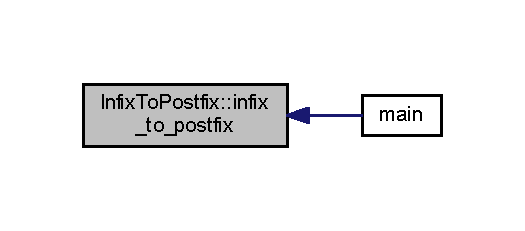
\includegraphics[width=252pt]{class_infix_to_postfix_a7206f78b3bb99dcba5bc4a8eb6fce5ad_icgraph}
\end{center}
\end{figure}


The documentation for this class was generated from the following file\+:\begin{DoxyCompactItemize}
\item 
\mbox{\hyperlink{_infix_to_postfix_8cpp}{Infix\+To\+Postfix.\+cpp}}\end{DoxyCompactItemize}

\hypertarget{class_inorder_traversal}{}\section{Inorder\+Traversal Class Reference}
\label{class_inorder_traversal}\index{Inorder\+Traversal@{Inorder\+Traversal}}


Contains the functions to convert postfix expression to rooted binary parse tree and a funtion to traverse the parse tree.  


\subsection*{Classes}
\begin{DoxyCompactItemize}
\item 
struct \mbox{\hyperlink{struct_inorder_traversal_1_1node}{node}}
\begin{DoxyCompactList}\small\item\em struct to represent a node of the parse tree \end{DoxyCompactList}\end{DoxyCompactItemize}
\subsection*{Static Public Member Functions}
\begin{DoxyCompactItemize}
\item 
static struct \mbox{\hyperlink{struct_inorder_traversal_1_1node}{node}} $\ast$ \mbox{\hyperlink{class_inorder_traversal_afdc83589caa4e0b0fe266cd147ed80c4}{new\+Node}} (char val)
\begin{DoxyCompactList}\small\item\em Intializes a node with a value. \end{DoxyCompactList}\item 
static void \mbox{\hyperlink{class_inorder_traversal_a0997a41c18ddf565f5f460446ef3c8a2}{postfix\+\_\+to\+\_\+parse\+\_\+tree}} (string postfix)
\begin{DoxyCompactList}\small\item\em Converts postfix propostional logic expression to rooted binary parse tree and then calls the traversal function. \end{DoxyCompactList}\item 
static void \mbox{\hyperlink{class_inorder_traversal_a9027f549ca60732409dbe4387785e0a4}{traverse\+\_\+parse}} (\mbox{\hyperlink{struct_inorder_traversal_1_1node}{node}} $\ast$cur)
\begin{DoxyCompactList}\small\item\em Prints the in-\/order traversal of the parse tree. \end{DoxyCompactList}\end{DoxyCompactItemize}


\subsection{Detailed Description}
Contains the functions to convert postfix expression to rooted binary parse tree and a funtion to traverse the parse tree. 

\subsection{Member Function Documentation}
\mbox{\Hypertarget{class_inorder_traversal_afdc83589caa4e0b0fe266cd147ed80c4}\label{class_inorder_traversal_afdc83589caa4e0b0fe266cd147ed80c4}} 
\index{Inorder\+Traversal@{Inorder\+Traversal}!new\+Node@{new\+Node}}
\index{new\+Node@{new\+Node}!Inorder\+Traversal@{Inorder\+Traversal}}
\subsubsection{\texorpdfstring{new\+Node()}{newNode()}}
{\footnotesize\ttfamily static struct \mbox{\hyperlink{struct_inorder_traversal_1_1node}{node}}$\ast$ Inorder\+Traversal\+::new\+Node (\begin{DoxyParamCaption}\item[{char}]{val }\end{DoxyParamCaption})\hspace{0.3cm}{\ttfamily [inline]}, {\ttfamily [static]}}



Intializes a node with a value. 


\begin{DoxyParams}{Parameters}
{\em val} & value with which the node is to be initialized \\
\hline
\end{DoxyParams}
\begin{DoxyReturn}{Returns}
node initialized with the value 
\end{DoxyReturn}
Here is the caller graph for this function\+:\nopagebreak
\begin{figure}[H]
\begin{center}
\leavevmode
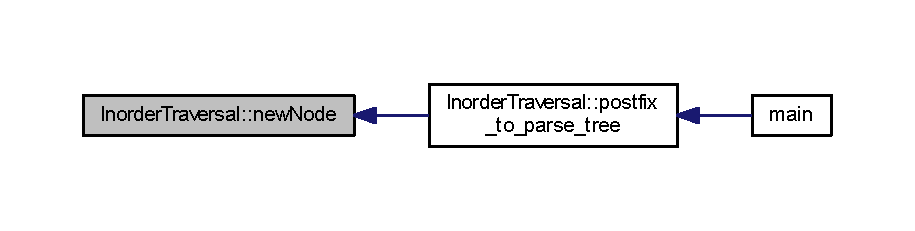
\includegraphics[width=350pt]{class_inorder_traversal_afdc83589caa4e0b0fe266cd147ed80c4_icgraph}
\end{center}
\end{figure}
\mbox{\Hypertarget{class_inorder_traversal_a0997a41c18ddf565f5f460446ef3c8a2}\label{class_inorder_traversal_a0997a41c18ddf565f5f460446ef3c8a2}} 
\index{Inorder\+Traversal@{Inorder\+Traversal}!postfix\+\_\+to\+\_\+parse\+\_\+tree@{postfix\+\_\+to\+\_\+parse\+\_\+tree}}
\index{postfix\+\_\+to\+\_\+parse\+\_\+tree@{postfix\+\_\+to\+\_\+parse\+\_\+tree}!Inorder\+Traversal@{Inorder\+Traversal}}
\subsubsection{\texorpdfstring{postfix\+\_\+to\+\_\+parse\+\_\+tree()}{postfix\_to\_parse\_tree()}}
{\footnotesize\ttfamily static void Inorder\+Traversal\+::postfix\+\_\+to\+\_\+parse\+\_\+tree (\begin{DoxyParamCaption}\item[{string}]{postfix }\end{DoxyParamCaption})\hspace{0.3cm}{\ttfamily [inline]}, {\ttfamily [static]}}



Converts postfix propostional logic expression to rooted binary parse tree and then calls the traversal function. 


\begin{DoxyParams}{Parameters}
{\em postfix} & the postfix propositional logic expression \\
\hline
\end{DoxyParams}
\begin{DoxyReturn}{Returns}
Void 
\end{DoxyReturn}
Here is the call graph for this function\+:\nopagebreak
\begin{figure}[H]
\begin{center}
\leavevmode
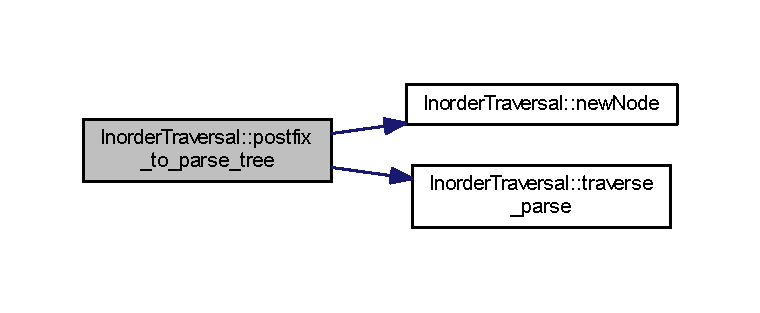
\includegraphics[width=350pt]{class_inorder_traversal_a0997a41c18ddf565f5f460446ef3c8a2_cgraph}
\end{center}
\end{figure}
Here is the caller graph for this function\+:\nopagebreak
\begin{figure}[H]
\begin{center}
\leavevmode
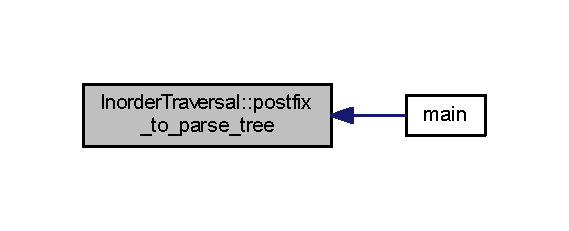
\includegraphics[width=273pt]{class_inorder_traversal_a0997a41c18ddf565f5f460446ef3c8a2_icgraph}
\end{center}
\end{figure}
\mbox{\Hypertarget{class_inorder_traversal_a9027f549ca60732409dbe4387785e0a4}\label{class_inorder_traversal_a9027f549ca60732409dbe4387785e0a4}} 
\index{Inorder\+Traversal@{Inorder\+Traversal}!traverse\+\_\+parse@{traverse\+\_\+parse}}
\index{traverse\+\_\+parse@{traverse\+\_\+parse}!Inorder\+Traversal@{Inorder\+Traversal}}
\subsubsection{\texorpdfstring{traverse\+\_\+parse()}{traverse\_parse()}}
{\footnotesize\ttfamily static void Inorder\+Traversal\+::traverse\+\_\+parse (\begin{DoxyParamCaption}\item[{\mbox{\hyperlink{struct_inorder_traversal_1_1node}{node}} $\ast$}]{cur }\end{DoxyParamCaption})\hspace{0.3cm}{\ttfamily [inline]}, {\ttfamily [static]}}



Prints the in-\/order traversal of the parse tree. 


\begin{DoxyParams}{Parameters}
{\em cur} & the root of the parse tree \\
\hline
\end{DoxyParams}
\begin{DoxyReturn}{Returns}
Void 
\end{DoxyReturn}
Here is the caller graph for this function\+:\nopagebreak
\begin{figure}[H]
\begin{center}
\leavevmode
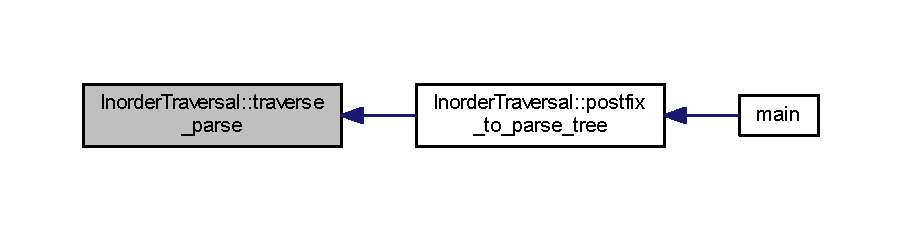
\includegraphics[width=350pt]{class_inorder_traversal_a9027f549ca60732409dbe4387785e0a4_icgraph}
\end{center}
\end{figure}


The documentation for this class was generated from the following file\+:\begin{DoxyCompactItemize}
\item 
\mbox{\hyperlink{_inorder_traversal_8cpp}{Inorder\+Traversal.\+cpp}}\end{DoxyCompactItemize}

\hypertarget{struct_inorder_traversal_1_1node}{}\section{Inorder\+Traversal\+:\+:node Struct Reference}
\label{struct_inorder_traversal_1_1node}\index{Inorder\+Traversal\+::node@{Inorder\+Traversal\+::node}}


struct to represent a node of the parse tree  




Collaboration diagram for Inorder\+Traversal\+:\+:node\+:\nopagebreak
\begin{figure}[H]
\begin{center}
\leavevmode
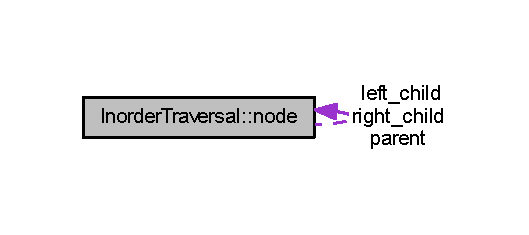
\includegraphics[width=254pt]{struct_inorder_traversal_1_1node__coll__graph}
\end{center}
\end{figure}
\subsection*{Public Attributes}
\begin{DoxyCompactItemize}
\item 
struct \mbox{\hyperlink{struct_inorder_traversal_1_1node}{node}} $\ast$ \mbox{\hyperlink{struct_inorder_traversal_1_1node_aa58b614b269c3b4d3b9240165d820b14}{parent}}
\item 
char \mbox{\hyperlink{struct_inorder_traversal_1_1node_ad27be9fbd1238d856d52eddcb61f8563}{val}}
\item 
struct \mbox{\hyperlink{struct_inorder_traversal_1_1node}{node}} $\ast$ \mbox{\hyperlink{struct_inorder_traversal_1_1node_abe2033bf83816d4df11f247bc739440b}{left\+\_\+child}}
\item 
struct \mbox{\hyperlink{struct_inorder_traversal_1_1node}{node}} $\ast$ \mbox{\hyperlink{struct_inorder_traversal_1_1node_ac6e7ee4328d89ecf0529a8ef5d6fedf9}{right\+\_\+child}}
\end{DoxyCompactItemize}


\subsection{Detailed Description}
struct to represent a node of the parse tree 

\subsection{Member Data Documentation}
\mbox{\Hypertarget{struct_inorder_traversal_1_1node_abe2033bf83816d4df11f247bc739440b}\label{struct_inorder_traversal_1_1node_abe2033bf83816d4df11f247bc739440b}} 
\index{Inorder\+Traversal\+::node@{Inorder\+Traversal\+::node}!left\+\_\+child@{left\+\_\+child}}
\index{left\+\_\+child@{left\+\_\+child}!Inorder\+Traversal\+::node@{Inorder\+Traversal\+::node}}
\subsubsection{\texorpdfstring{left\+\_\+child}{left\_child}}
{\footnotesize\ttfamily struct \mbox{\hyperlink{struct_inorder_traversal_1_1node}{node}}$\ast$ Inorder\+Traversal\+::node\+::left\+\_\+child}

\mbox{\Hypertarget{struct_inorder_traversal_1_1node_aa58b614b269c3b4d3b9240165d820b14}\label{struct_inorder_traversal_1_1node_aa58b614b269c3b4d3b9240165d820b14}} 
\index{Inorder\+Traversal\+::node@{Inorder\+Traversal\+::node}!parent@{parent}}
\index{parent@{parent}!Inorder\+Traversal\+::node@{Inorder\+Traversal\+::node}}
\subsubsection{\texorpdfstring{parent}{parent}}
{\footnotesize\ttfamily struct \mbox{\hyperlink{struct_inorder_traversal_1_1node}{node}}$\ast$ Inorder\+Traversal\+::node\+::parent}

\mbox{\Hypertarget{struct_inorder_traversal_1_1node_ac6e7ee4328d89ecf0529a8ef5d6fedf9}\label{struct_inorder_traversal_1_1node_ac6e7ee4328d89ecf0529a8ef5d6fedf9}} 
\index{Inorder\+Traversal\+::node@{Inorder\+Traversal\+::node}!right\+\_\+child@{right\+\_\+child}}
\index{right\+\_\+child@{right\+\_\+child}!Inorder\+Traversal\+::node@{Inorder\+Traversal\+::node}}
\subsubsection{\texorpdfstring{right\+\_\+child}{right\_child}}
{\footnotesize\ttfamily struct \mbox{\hyperlink{struct_inorder_traversal_1_1node}{node}}$\ast$ Inorder\+Traversal\+::node\+::right\+\_\+child}

\mbox{\Hypertarget{struct_inorder_traversal_1_1node_ad27be9fbd1238d856d52eddcb61f8563}\label{struct_inorder_traversal_1_1node_ad27be9fbd1238d856d52eddcb61f8563}} 
\index{Inorder\+Traversal\+::node@{Inorder\+Traversal\+::node}!val@{val}}
\index{val@{val}!Inorder\+Traversal\+::node@{Inorder\+Traversal\+::node}}
\subsubsection{\texorpdfstring{val}{val}}
{\footnotesize\ttfamily char Inorder\+Traversal\+::node\+::val}



The documentation for this struct was generated from the following file\+:\begin{DoxyCompactItemize}
\item 
\mbox{\hyperlink{_inorder_traversal_8cpp}{Inorder\+Traversal.\+cpp}}\end{DoxyCompactItemize}

\chapter{File Documentation}
\hypertarget{_infix_to_postfix_8cpp}{}\section{Infix\+To\+Postfix.\+cpp File Reference}
\label{_infix_to_postfix_8cpp}\index{Infix\+To\+Postfix.\+cpp@{Infix\+To\+Postfix.\+cpp}}
{\ttfamily \#include $<$bits/stdc++.\+h$>$}\newline
Include dependency graph for Infix\+To\+Postfix.\+cpp\+:\nopagebreak
\begin{figure}[H]
\begin{center}
\leavevmode
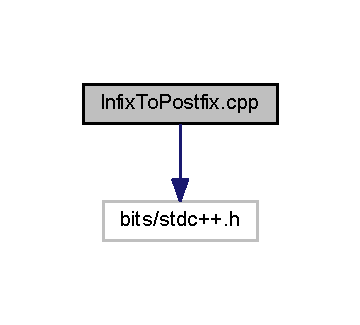
\includegraphics[width=173pt]{_infix_to_postfix_8cpp__incl}
\end{center}
\end{figure}
This graph shows which files directly or indirectly include this file\+:\nopagebreak
\begin{figure}[H]
\begin{center}
\leavevmode
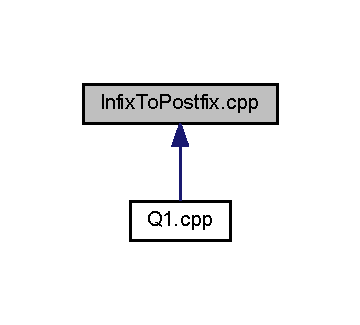
\includegraphics[width=173pt]{_infix_to_postfix_8cpp__dep__incl}
\end{center}
\end{figure}
\subsection*{Classes}
\begin{DoxyCompactItemize}
\item 
class \mbox{\hyperlink{class_infix_to_postfix}{Infix\+To\+Postfix}}
\begin{DoxyCompactList}\small\item\em Contains the function to convert infix expression to postfix expression. \end{DoxyCompactList}\end{DoxyCompactItemize}

\hypertarget{_inorder_traversal_8cpp}{}\section{Inorder\+Traversal.\+cpp File Reference}
\label{_inorder_traversal_8cpp}\index{Inorder\+Traversal.\+cpp@{Inorder\+Traversal.\+cpp}}
{\ttfamily \#include $<$bits/stdc++.\+h$>$}\newline
Include dependency graph for Inorder\+Traversal.\+cpp\+:\nopagebreak
\begin{figure}[H]
\begin{center}
\leavevmode
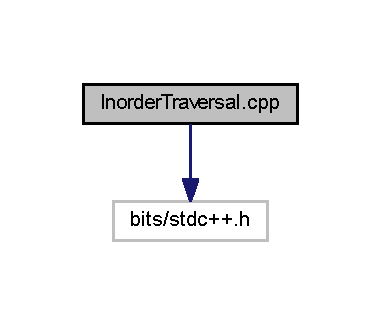
\includegraphics[width=183pt]{_inorder_traversal_8cpp__incl}
\end{center}
\end{figure}
This graph shows which files directly or indirectly include this file\+:\nopagebreak
\begin{figure}[H]
\begin{center}
\leavevmode
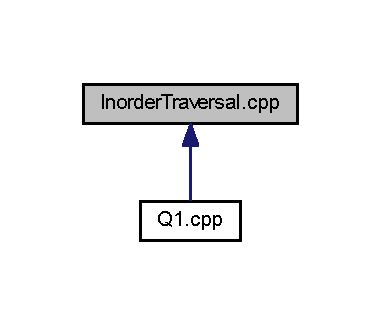
\includegraphics[width=183pt]{_inorder_traversal_8cpp__dep__incl}
\end{center}
\end{figure}
\subsection*{Classes}
\begin{DoxyCompactItemize}
\item 
class \mbox{\hyperlink{class_inorder_traversal}{Inorder\+Traversal}}
\begin{DoxyCompactList}\small\item\em Contains the functions to convert postfix expression to rooted binary parse tree and a funtion to traverse the parse tree. \end{DoxyCompactList}\item 
struct \mbox{\hyperlink{struct_inorder_traversal_1_1node}{Inorder\+Traversal\+::node}}
\begin{DoxyCompactList}\small\item\em struct to represent a node of the parse tree \end{DoxyCompactList}\end{DoxyCompactItemize}

\hypertarget{mainpage_8cpp}{}\section{mainpage.\+cpp File Reference}
\label{mainpage_8cpp}\index{mainpage.\+cpp@{mainpage.\+cpp}}

\hypertarget{_q1_8cpp}{}\section{Q1.\+cpp File Reference}
\label{_q1_8cpp}\index{Q1.\+cpp@{Q1.\+cpp}}
{\ttfamily \#include $<$bits/stdc++.\+h$>$}\newline
{\ttfamily \#include \char`\"{}Infix\+To\+Postfix.\+cpp\char`\"{}}\newline
{\ttfamily \#include \char`\"{}Inorder\+Traversal.\+cpp\char`\"{}}\newline
Include dependency graph for Q1.\+cpp\+:\nopagebreak
\begin{figure}[H]
\begin{center}
\leavevmode
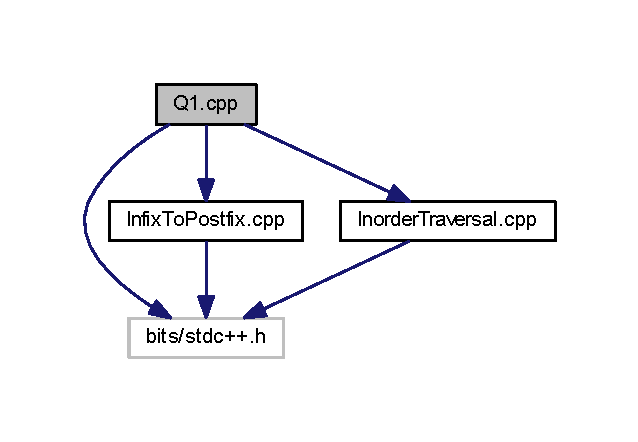
\includegraphics[width=306pt]{_q1_8cpp__incl}
\end{center}
\end{figure}
\subsection*{Functions}
\begin{DoxyCompactItemize}
\item 
int \mbox{\hyperlink{_q1_8cpp_ae66f6b31b5ad750f1fe042a706a4e3d4}{main}} ()
\end{DoxyCompactItemize}


\subsection{Function Documentation}
\mbox{\Hypertarget{_q1_8cpp_ae66f6b31b5ad750f1fe042a706a4e3d4}\label{_q1_8cpp_ae66f6b31b5ad750f1fe042a706a4e3d4}} 
\index{Q1.\+cpp@{Q1.\+cpp}!main@{main}}
\index{main@{main}!Q1.\+cpp@{Q1.\+cpp}}
\subsubsection{\texorpdfstring{main()}{main()}}
{\footnotesize\ttfamily int main (\begin{DoxyParamCaption}{ }\end{DoxyParamCaption})}

Here is the call graph for this function\+:\nopagebreak
\begin{figure}[H]
\begin{center}
\leavevmode
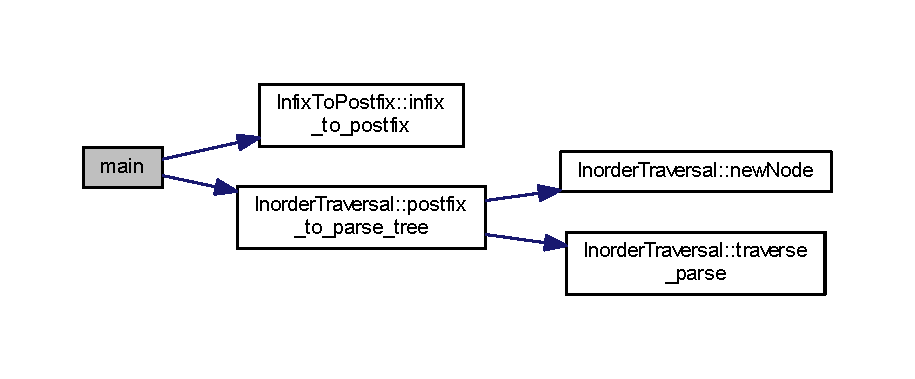
\includegraphics[width=350pt]{_q1_8cpp_ae66f6b31b5ad750f1fe042a706a4e3d4_cgraph}
\end{center}
\end{figure}

%--- End generated contents ---

% Index
\backmatter
\newpage
\phantomsection
\clearemptydoublepage
\addcontentsline{toc}{chapter}{Index}
\printindex

\end{document}
